% Appendix A

\chapter{Script principal} % Main appendix title

\label{Script principal}

El script principal del proyecto contiene un procesador de líneas de comando que facilita la ejecución de los diferentes casos de uso. Los usos básicos del procesador se detallan a continuación:

\begin{itemize}
    \item Mostrar la ayuda.
\end{itemize}
\begin{verbatim}
$ python -m src.main --help
\end{verbatim}

\begin{itemize}
    \item Jugar al Tetris con el teclado.
\end{itemize}
\begin{verbatim}
$ python -m src.main play --human
\end{verbatim}

\begin{itemize}
    \item Entrenar un nuevo agente de Double-DQN.
\end{itemize}
\begin{verbatim}
$ python -m src.main train --model=ddqn
\end{verbatim}

\begin{itemize}
    \item Entrenar un nuevo agente de Dueling-DQN.
\end{itemize}
\begin{verbatim}
$ python -m src.main train --model=dueling-dqn
\end{verbatim}

\begin{itemize}
    \item Ejecutar el juego Tetris con un agente Double-DQN entrenado.
\end{itemize}
\begin{verbatim}
$ python -m src.main play \
    --model-file="./resources/ddqn/model_ddqn.pkl" --model=ddqn
\end{verbatim}

\begin{itemize}
    \item Ejecutar el juego Tetris con un agente Dueling-DQN entrenado.
\end{itemize}
\begin{verbatim}
$ python -m src.main play \
    --model-file="./resources/dueling_dqn/model_dueling_dqn.pkl" \
    --model=dueling-dqn
\end{verbatim}

\begin{figure}[htbp]
	\centering
	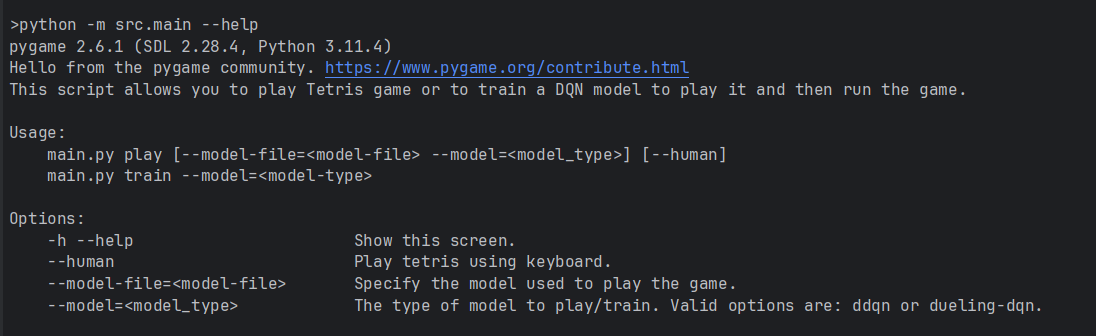
\includegraphics[width=\textwidth]{./Figures/command.png}
	\caption{Uso del script principal por línea de comando.}
	\label{fig:command}
\end{figure}